\documentclass{article}

\usepackage[left=2cm,right=2cm, top=2cm, bottom = 2cm]{geometry}
\usepackage{amsfonts}
\usepackage{amsmath}
%%%\usepackage{array}

\usepackage{tikz}

\pagestyle{empty}

%%%\setlength{\tabcolsep}{1.8cm}
%%%\renewcommand{\arraystretch}{2.5}

%%%\makeatletter
%%%\newcommand{\thickhline}{%
%%%    \noalign {\ifnum 0=`}\fi \hrule height 2pt
%%%    \futurelet \reserved@a \@xhline
%%%}
%%%\newcolumntype{!}{@{\hskip\tabcolsep\vrule width 2pt\hskip\tabcolsep}}
%%%\makeatother

\begin{document}

\title{Circles and Tangents}
\date{}

\maketitle
\thispagestyle{empty}

\Large

\section{Key Properties}

\begin{enumerate}
	\item Write down the equation of the circle with centre $(-1,4)$ and radius 7.
	\item Give the centre and radius of the circle with equation $(x-2)^2+(y+9)^2-25=0$.
	\item Consider the circle below, in which $O$ is the center.
		\begin{center}
		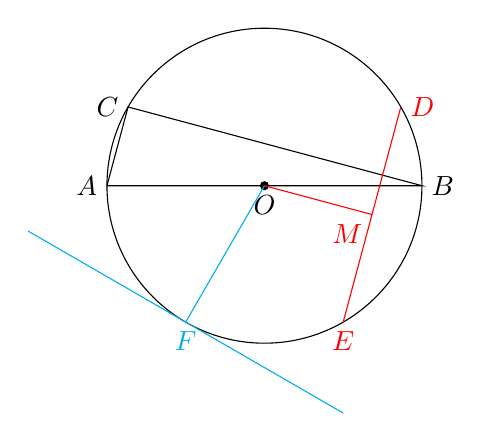
\begin{tikzpicture}
			\draw (-2,0) -- (2,0) -- (-1.732,1) -- (-2,0);
			\node[left] at (-2,0) {$A$};
			\node[right] at (2,0) {$B$};
			\node[left] at (-1.732,1) {$C$};
			\draw (0,0) circle[radius=2];
			\draw[fill] (0,0) circle[radius=0.05];
			\node[below] at (0,0) {$O$};
			
			\draw[red] (1.732,1) -- (1,-1.732);
			\node[right,red] at (1.732,1) {$D$};
			\node[below,red] at (1,-1.732) {$E$};
			\node[below left,red] at (1.366,-0.366) {$M$};
			\draw[red] (1.366,-0.366) -- (0,0);

			\draw[cyan] (-1,-1.732) -- (0,0);
			\node[below,cyan] at (-1,-1.732) {$F$};
			\draw[cyan] (-3,-0.577) -- (1,-2.887);
			% x^2+y^2=4. 2x + 2yy' = 0. y'=-x/y. y=(-1/1.732)(x+1)-1.732. x=-3: y=2/1.732-1.732=-0.577. x=1, y=-2/1.732-1.732=-2.887
		\end{tikzpicture}
		\end{center}
		
		\begin{enumerate}
			\item What is the angle $ACB$?
			{\color{red}\item The line $OM$ is perpendicular to the line $DE$. In what ratio does $OM$ divide $DE$?}
			{\color{cyan}\item The cyan line is tangent to the circle at $F$. What angle does it make with the radius $OF$?}
		\end{enumerate}
\end{enumerate}



\clearpage



\section{Practice Questions}


\begin{enumerate}
	\item Find the radius and centre of the circle with equation $x^2+7x-8y+y^2-30=0$.
	\item In the diagram below, $O$ is the origin, $A$ has coordinates $(2,0)$, angle $AOB$ is $40^\circ$, and line $OB$ has length 7. The circle $C$ passes through $O$, $A$, and $B$.
		\begin{center}
		\begin{tikzpicture}
			\draw[->] (-3,0) -- (6,0);
			\node[right] at (6,0) {$x$};
			\draw[->] (0,0) -- (0,8);
			\node[above] at (0,8) {$y$};
			
			\node[below left] at (0,0) {$O$};
			\node[below] at (2,0) {$A$};
			\draw (0,0) -- (5,4) -- (2,0);
			\node[above right] at (5,4) {$B$};
			\node[above left] at (2.5,2) {$7$};
			\node[above right] at (0.5,0) {$40^\circ$};
			\node[below] at (1,0) {2};
			
			\draw (1,3.875) circle [radius=4];
			\node[right] at (-3,3.875) {$C$};
		\end{tikzpicture}
		\end{center}
		
		\begin{enumerate}
			\item Find the coordinates of $B$. % (7cos(40^\circ), 7\sin(40^\circ)) \approx (5.36,4.5)  REAL: (5,4)
			\item Find the equations of the perpendicular bisectors of $OA$ and $OB$. % OA: x=1. OB: y=(-4.5/5.36)(x-2.68)+2.25.  REAL: x=1, y=-1.25(x-2.5)+2
			\item Hence find the coordinates of the center of the circle $C$. % x=1, y=-4.5/5.36 + 4.5 \approx 3.66. REAL: x=1, y=1.25*1.5 + 2 = 3.875
			\item Hence find the equation of $C$. % r=\sqrt{1+3.66^2}\approx 3.79. REAL: sqrt{1+3.875^2}\approx 4.002
		\end{enumerate}
	\item Let $C$ be the circle with centre $(-3,4)$ and radius $5$.
		\begin{enumerate}
			\item Show that $(0,0)$ lies on $C$.
			\item Find the equation of the tangent to $C$ at $(0,0)$.
		\end{enumerate}
	\item The circle $C$ has centre $A$ with coordinates $(7,5)$. The line with equation $y=2x+1$ is tangent to $C$ at $P$.
		\begin{enumerate}
			\item Show that the line $PA$ has equation $2y+x=17$.
			\item Hence find the coordinates of $P$.
			\item Hence find an equation of $C$.
			\item The line $y=2x+k$ is also tangent to $C$, where $k\neq 1$ is a constant. Find the value of $k$.
		\end{enumerate}
\end{enumerate}


\end{document}